\documentclass{article}

\usepackage[english]{babel}
\usepackage[utf8]{inputenc}
\usepackage{amsmath,amssymb}
\usepackage{parskip}
\usepackage{graphicx}

% Margins
\usepackage[top=2.5cm, left=3cm, right=3cm, bottom=4.0cm]{geometry}
% Colour table cells
\usepackage[table]{xcolor}

% Get larger line spacing in table
\newcommand{\tablespace}{\\[1.25mm]}
\newcommand\Tstrut{\rule{0pt}{2.6ex}}         % = `top' strut
\newcommand\tstrut{\rule{0pt}{2.0ex}}         % = `top' strut
\newcommand\Bstrut{\rule[-0.9ex]{0pt}{0pt}}   % = `bottom' strut

\renewcommand\thesubsubsection{\alph{subsubsection}.)}

\title{COS333 Practical 1}
\author{Dylan Kapnias \\ u18108467}

\begin{document}
\maketitle

\section{Research Questions}
\subsection{}
An esoteric programming language is a programming language that has been designed not for practical use, but rather as a language meant for experimentation or as a fun joke project \cite{web:eso:def}.

\subsection{}
\subsubsection{}
Advantage:- 
\linebreak{}
\linebreak{}
Disadvantage:- One of the disadvantages with all of the Funges family of languages (with the exception of Befunges-98), is the limit to the size of the playfield (the space in which code can be entered), thus making these languages not able to be Turing-complete.

\subsubsection{}
Advantage:- 
\linebreak{}
\linebreak{}
Disadvantage:-

\subsection{}
\underline{\textbf{brainfuck}}
\linebreak{}
This language was invented by Urban Müller in 1993, whilst attempting to make a language such that he could write the smallest possible compiler for the version 2.0 of Amiga OS \cite{web:brainfuck:def}. There is not much to the language in terms of syntax as other than the characters $><+-.,[]$ everything else is considered a comment, and thus is ignored. Semantically the language is Turing-complete and operates by manipulating an array of memory cells. The following is a simple "Hello World!" in this language:-
\begin{verbatim}
++++++++[>++++[>++>+++>+++>+<<<<-]>+>+>->>+[<]<-]>>.>---.+++++++..+++.>>.<-.<.+++.---
---.--------.>>+.>++.
\end{verbatim}

\linebreak{}
\linebreak{}

\underline{\textbf{Piet}}
\linebreak{}
This language was invented by David Morgan-Mar, who name the language after a pioneer in the sphere of geometrical abstract art, Piet Mondrian \cite{web:piet:def}. The syntax of the language is quite interesting due to the fact that the way to input instructions is through the use of the 20 colours that the language supports. Semantically the language is Turing-complete and operates by controlling and manipulating a stack of integer values. All the colours are cyclically linked and thus the instructions for the stack manipulation are determined through the transition of the colours as the interpreter flows through the program. The following figure is of a simple "Hello World!" program in this language:-
\linebreak{}
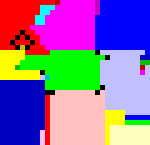
\includegraphics{Piet_hello_big.png}

\linebreak{}
\linebreak{}

\subsection{}
Design by contract is a way of software design that focuses on specifying contracts of interaction between the components of the system, assuming that the components interact with each other in a client-server model of architecture. Thus, the contract between the client and the server provides the client the assurance that the server will uphold it's promises as long as both the server and the client abide by the postconditions and the invariants set on the contract. Due to these contracts essentially just being assertions, the esolangs Daft and ComeFrom2 should also have native support design by contract.

\pagebreak

\bibliographystyle{plain}
\bibliography{references}

\end{document}
